\chapter{Properties}
\paragraph{} After 5 days of running from the goose police, Duckie was certain that he had escaped. He decided to stop for dinner, but just as he took off, \textbf{Squak!} He ran headfirst into another goose. 
\paragraph{} "Hold it right there! You need to come back with me to the village!" the policegoose demanded, slightly dazed. 
\paragraph{} "It's dangerous in the outside world. This is for your own safety!"
\paragraph{} Duckie knew that the policegoose, named Güs, was a fair goose, and so considered this for a moment. "Of course it's dangerous! But I have to do this. I am looking for the golden goose of legend. The one who is supposed to save us, change all of goose society and help us through our migrations."
\paragraph{} "Oh. Hmm, that makes sense. But why are the goose authorities trying to stop you? Isn't your cause noble?" Güs asked.
\paragraph{} "They are afraid. If I can find the golden goose, then they may not be able to stay in power. You joined the goose police to help people, and if you let me go, you can do just that!"
\paragraph{} "Your cause is noble, and I would like to help, but if I just let you go without at least trying to stop you, I will get in trouble! I'll tell you what. I will have a series of challenges with you. If you beat me in all the challenges, I will let you go. If not, you have to let me take you back. Sound fair?"
\paragraph{} Duckie was reluctant, but knew that he had no other options. "Fine. Let's do the challenges."
\pagebreak
%Associativity
\subchapter{Associativity}
{Güs and Duckie both thought they were good flyers, so they decided to compete in a three-part flying distance competition. The first leg of the race was \textbf{4} km, the second leg was \textbf{3} km, and the third leg was \textbf{1} km. The distance flying competition rules stated that any goose would be allowed to take one break in between laps. They both wanted to win, so created strategies. Güs decided to travel the first leg (\textbf{4} km) of the race, took his break then travel the second and third legs (\textbf{3} km and \textbf{1} km). Duckie instead traveled the first leg, (\textbf{4} km) of the race and the second leg (\textbf{3} km) of the race, then took his break, and traveled the third leg (\textbf{1} km). Did they tie?}
{Yes! Duckie and Güs traveled the same amount.}
{When adding, computation can be grouped in any way. In other words: (A+B)+C = A+(B+C).}
{\begin{tikzpicture}
    \coordinate (A) at (0,0);
    \coordinate (B) at (0,4);
    \coordinate (C) at (0,7);
    \coordinate (D) at (0,8);
    \coordinate (Ap) at (1.5,0);
    \coordinate (Bp) at (1.5,4);
    \coordinate (Cp) at (1.5,7);
    \coordinate (Dp) at (1.5,8);
    
    \node [inner sep=0pt] at (D) {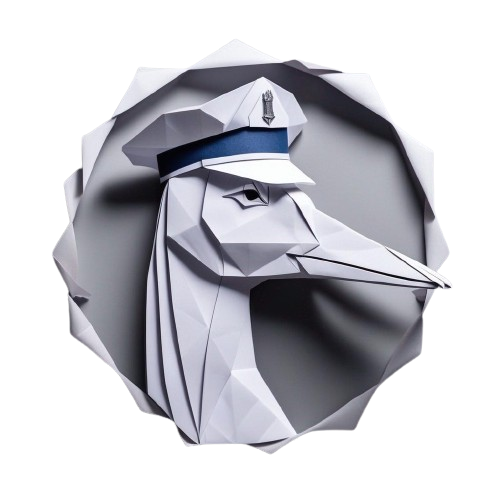
\includegraphics[height=0.8cm]{Gus}};
    \draw[-|,ultra thick,red, decorate, decoration={random steps,segment length=3pt,amplitude=0.2pt}] (A) -- (B) node[midway, left] {4 km};
    \draw[->,ultra thick,blue, decorate, decoration={random steps,segment length=3pt,amplitude=0.2pt}] (B) -- (C) node[midway, left] {3 km};
    \draw[->,ultra thick,violet, decorate, decoration={random steps,segment length=3pt,amplitude=0.2pt}] (C) -- (D) node[midway, left] {1 km};
    
    \node [inner sep=0pt] at (Dp) {
\includegraphics[height=0.8cm]{DuckieGami}};
    \draw[->,ultra thick,red, decorate, decoration={random steps,segment length=3pt,amplitude=0.2pt}] (Ap) -- (Bp) node[midway, left] {4 km};
    \draw[-|,ultra thick,blue, decorate, decoration={random steps,segment length=3pt,amplitude=0.2pt}] (Bp) -- (Cp) node[midway, left] {3 km};
    \draw[->,ultra thick,violet, decorate, decoration={random steps,segment length=3pt,amplitude=0.2pt}] (Cp) -- (Dp) node[midway, left] {1 km};
    
    \draw [decorate, 
	decoration = {brace,mirror,
		raise=15pt,}] (Ap) -- (Dp) node[midway, right, xshift=0.5cm] {27 km};
\end{tikzpicture}}
%Additive Commutativity
\subchapter{Additive Commutativity}
{Duckie and Güs decided that to break the tie, they needed to do another competition. \linebreak Because geese are water animals, swimming is a very important skill, so they decided that that should be their next competition. They each had a different strategy. Güs swam \textbf{140} m, dried off, then swam \textbf{160} m. Duckie instead swam \textbf{160} m, dried off, then swam \textbf{140} m. Did they tie?}
{Yes! Duckie and Güs swam the same amount.}
{The order of adding does not matter. In other words: A+B = B+A.}
{\begin{tikzpicture}
    \coordinate (A) at (0,0);
    \coordinate (B) at (0,4);
    \coordinate (C) at (0,9);
    \coordinate (Ap) at (1.5,0);
    \coordinate (Bp) at (1.5,5);
    \coordinate (Cp) at (1.5,9);
    
    \node [inner sep=0pt] at (C) {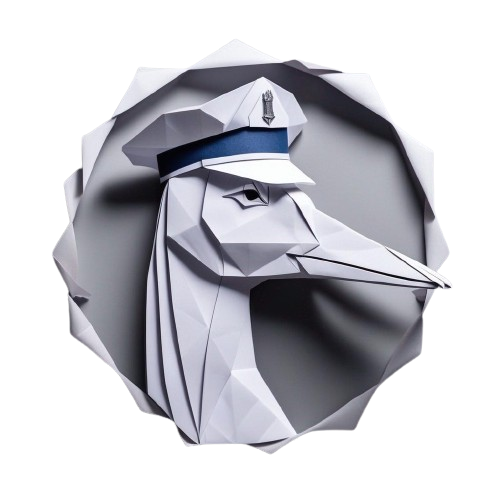
\includegraphics[height=0.8cm]{Gus}};
    \draw[->,ultra thick,red, decorate, decoration={random steps,segment length=3pt,amplitude=0.2pt}] (A) -- (B) node[midway, left] {140 m};
    \draw[->,ultra thick,blue, decorate, decoration={random steps,segment length=3pt,amplitude=0.2pt}] (B) -- (C) node[midway, left] {160 m};
    
    \node [inner sep=0pt] at (Cp) {
\includegraphics[height=0.8cm]{DuckieGami}};
    \draw[->,ultra thick,blue, decorate, decoration={random steps,segment length=3pt,amplitude=0.2pt}] (Ap) -- (Bp) node[midway, left] {160 m};
    \draw[->,ultra thick,red, decorate, decoration={random steps,segment length=3pt,amplitude=0.2pt}] (Bp) -- (Cp) node[midway, left] {140 m};
    
    \draw [decorate, 
	decoration = {calligraphic brace,mirror,
		raise=10pt,amplitude=5pt}] (Ap) -- (Cp) node[midway, right, xshift=0.5cm,line width=3pt] {300 m};
\end{tikzpicture}}
%Distributativity
\subchapter{Distributivity}
{Duckie and Güs were starting to get frustrated. No matter what happened, the seemed to tie every time! Duckie had thought that if he competed long enough, Güs would get tired and he would be able to win, so challenged him to another flying contest. In the third contest, Güs traveled \textbf{2} km, then \textbf{4} km, and repeated that pattern \textbf{2} times. Duckie instead traveled \textbf{2} km \textbf{2} times, then \textbf{4} km \textbf{2} times. Did they tie?}
{Yes! Duckie and Güs flew the same amount.}
{Multiplying by a full expression is the same as multiplying by each part of the expression. In other words: A*(B+C) = (A*B) + (A*C).}
{\begin{tikzpicture}
    \coordinate (A) at (0,0);
    \coordinate (B) at (0,4);
    \coordinate (C) at (0,9);
    \coordinate (Ap) at (1.5,0);
    \coordinate (Bp) at (1.5,5);
    \coordinate (Cp) at (1.5,9);
    
    \node [inner sep=0pt] at (C) {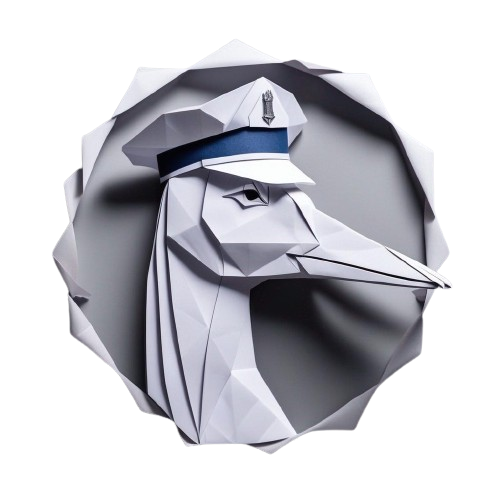
\includegraphics[height=0.8cm]{Gus}};
    \draw[->,ultra thick,red, decorate, decoration={random steps,segment length=3pt,amplitude=0.2pt}] (A) -- (B) node[midway, left] {140 m};
    \draw[->,ultra thick,blue, decorate, decoration={random steps,segment length=3pt,amplitude=0.2pt}] (B) -- (C) node[midway, left] {160 m};
    
    \node [inner sep=0pt] at (Cp) {
\includegraphics[height=0.8cm]{DuckieGami}};
    \draw[->,ultra thick,blue, decorate, decoration={random steps,segment length=3pt,amplitude=0.2pt}] (Ap) -- (Bp) node[midway, left] {160 m};
    \draw[->,ultra thick,red, decorate, decoration={random steps,segment length=3pt,amplitude=0.2pt}] (Bp) -- (Cp) node[midway, left] {140 m};
    
     \draw [decorate, 
	decoration = {calligraphic brace,mirror,
		raise=10pt,amplitude=5pt}] (Ap) -- (Cp) node[midway, right, xshift=0.5cm,line width=3pt] {300 m};
\end{tikzpicture}}
%Commutativity
\subchapter{Multiplicative Commutativity}
{At this point, Güs realized that Duckie was a very capable goose. When he first challenged Duckie, he expected winning to be a cakewalk, but his opponent ended up posing quite a challenge. Being an honorable goose, this made him respect Duckie more. He decided that the next contest should be a weightlifting competition, where whoever lifted the most amount of total weight would win. Duckie lifted \textbf{10} kg \textbf{3} times, whereas Güs lifted only \textbf{3} kg but does it \textbf{10} times. Did they tie?}
{Yes! Duckie and Güs lifted the same amount.}
{The order of multiplication does not affect the result. In other words: A * B = B * A.}
{\begin{tikzpicture} 
    \node [inner sep=0pt] at (0,15) {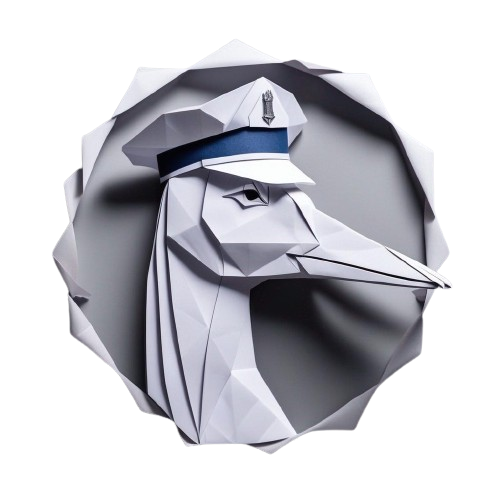
\includegraphics[height=0.8cm]{Gus}};
    \foreach \pos in {1,...,10} {	
        \MODULO{\pos}{2}{\rval}
        \SUBTRACT{\pos}{1}{\bl}
        \MODULO{\bl}{2}{\bval}
        \definecolor{col}{rgb}{\rval,0,\bval}
        \draw[->,ultra thick,col, decorate, decoration={random steps,segment length=3pt,amplitude=0.2pt}] (0,\pos *1.5 - 1.5) -- (0,\pos *1.5) node[midway, left] {3 kg};
    }
     \node [inner sep=0pt] at (1.5,15) {
\includegraphics[height=0.8cm]{DuckieGami}};
    \foreach \pos in {1,...,3} {	
        \MODULO{\pos}{2}{\rval}
        \SUBTRACT{\pos}{1}{\bl}
        \MODULO{\bl}{2}{\bval}
        \definecolor{col}{rgb}{\bval,\rval,\bval}
        \draw[->,ultra thick,col, decorate, decoration={random steps,segment length=3pt,amplitude=0.2pt}] (1.5,\pos *5 - 5) -- (1.5,\pos *5) node[midway, left] {10 kg};
    }
    
    \draw [decorate, decoration = {calligraphic brace,mirror, raise=10pt,amplitude=5pt}] (1.5,0) -- (1.5,15) node[midway, right, xshift=0.5cm,line width=3pt] {30 kg};
\end{tikzpicture}}
%End Of Chapter 2
\paragraph{} After the competition, Duckie and Güs sat down, exhausted. They had both realized that, no matter what competition they had, they were equally matched. Neither one would be able to beat the other, and they had won each other's respect. 
\paragraph{} "Why don't you join me?" asked Duckie.
\paragraph{} "I can't!" Güs cried. "What about my life in the goose police?"
\paragraph{} "Well, do you believe the golden goose is out there?"
\paragraph{} "Honestly, I'm not sure, but if the stories are true, it could change the world."
\paragraph{} Duckie agreed. He knew that there was the possibility the golden goose was a hoax, but believed the positive implications outweighed the dangers of disobeying the goose authorities. 
\paragraph{} "You joined the goose police to help people", he reasoned. "You are clearly strong and capable of making the dangerous journey, and if you can join me, you could do exactly that."
\paragraph{} Güs knew he was right. While he was afraid of what could happen along the journey, he decided to be brave and join Duckie. 
\paragraph{} "All right. I will join you!" he said resolutely. 